\subsection{Basics}
\paragraph{Definition}
It is an hidden Markov models, except the hidden states are continuous.
The model can be written in the following generic form: 
\fr{$\begin{cases}
    \bm{z}_{t} = g(\bm{u}_{t}, \bm{z}_{t-1}, \bm{\epsilon}_{t}) \\
    \bm{y}_{t} = h(\bm{z}_{t}, \bm{u}_{t-1}, \bm{\delta}_{t})
\end{cases}$}
where $\bm{z}_{t}$ is the hidden state $\bm{u}_{t}$ is an optimal input or control signal, $\bm{y}_{
t}$ is the observation is the \emph{transition model}, $h$ is the \emph{observation model} and $\bm{
\epsilon}_{t}$ is the system noise at time $t$.
\begin{itemize}
    \item \emph{transition model}: $\bm{z}_{t} = \bm{A}_{t}\bm{z}_{t-1} + \bm{B}_{t}\bm{u}_{t} +
        \bm{\epsilon}_{t}$
    \item \emph{observation model} $\bm{y}_{t} = \bm{C}_{t}\bm{z}_{t} + \bm{D}_{t}\bm{u}_{t} + \bm{
        \epsilon}_{t}$
    \item \emph{system noise}: $\bm{\epsilon}_{t}\hookrightarrow \mathcal{N}(\bm{0}, \bm{Q}_{t})$
    \item \emph{observation noise}: $\bm{\delta}_{t}\hookrightarrow \mathcal{N}(\bm{0}, \bm{R}_{t})$
\end{itemize}

\subsection{Time Series Forecasting}
The idea is to create a generative model of the data in terms of latent processes which capture 
different aspects of the signal.

\paragraph{Local level model}
The simplest latent process:
$\begin{cases}
    y_{t} &= a_{t} + \epsilon^{y}_{t},~\epsilon^{y}_{t}\hookrightarrow \mathcal{N}(0, R)\\
    a_{t} &= a_{t-1} + \epsilon^{a}_{t},~\epsilon^{a}_{t}\hookrightarrow \mathcal{N}(0, Q)
\end{cases}$
where the hidden state is just $z_{t}=a_{t}$
\paragraph{Local linear trend}
Many time series exhibit linear trends upward or downward, at least locally. We can model this by
letting the level $a_{t}$ change by an amount $b_{t}$ at each step :
$\begin{cases}
    y_{t} &= a_{t} + \epsilon^{y}_{t},~\epsilon^{y}_{t}\hookrightarrow \mathcal{N}(0, R)\\
    a_{t} &= a_{t-1} + b_{t-1} + \epsilon^{a}_{t},~\epsilon^{a}_{t}\hookrightarrow \mathcal{N}(0, 
    Q_{a})\\
    b_{t} &= b_{t-1} + \epsilon^{b}_{t},~\epsilon^{b}_{t}\hookrightarrow \mathcal{N}(0, Q_{b})
\end{cases}$
\paragraph{Seasonality}
This can be modeled by adding a latent process consisting of a series offset terms $c_{t}$ which
sum to zero (on average) over a complete cycle of $S$ steps:
$c_{t} = -\su{s=1}{S-1}c_{t-s}+\epsilon^{c}_{t}, \epsilon^{c}_{t}\hookrightarrow\mathcal{N}(0, 
Q_{c})$

\paragraph{ARMA(Auto-Regressive Moving-Average) models}
$x_{t} = \su{i=1}{p}\alpha_{i}x_{t-i} + \su{j=1}{q}\beta_{j}w_{t-j}+v_{t}$, where $v_{t}$ and $w_{t}$
follow a $\mathcal{N}(0, 1)$
\begin{figure}[H]
    \begin{center}
        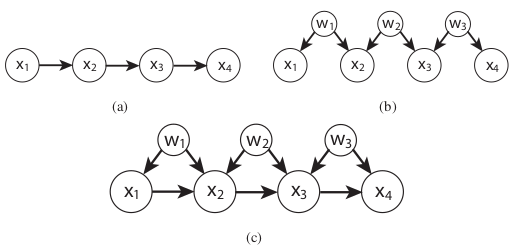
\includegraphics[width=.5\textwidth]{./chapters/2_statistics/07_hidden_markov_models/2_images/1_arma_graph.png}
    \end{center}
    \caption{(a)$\rightarrow~AR(1)$ (b)$\rightarrow~MA(1)$ and (c)$\rightarrow~ARMA(1,1)$}
    \label{fig:1_arma_graph}
\end{figure}
The structural approach to time series is often easier to understand than the ARMA approach.
In addition it allows the parameters to evolve over time, which makes the models more adaptive to 
non-stationary.

\subsection{Inference in LG-SSM (Linear Gaussian - State Space Models)}
\paragraph{Kalman filtering algorithm}
It is Kalman filter is an \tB{algorithm for exact Bayesian filtering for linear-Gaussian 
state space models} that sequentially computes $\prob{\bm{z}_{t}|\left(\bm{y}_{k}
\right)_{1\leq k\leq t}}$ for each $t$.

\subparagraph{Prediction step}
\begin{align*}
    \prob{\bm{z}_{t}|\bm{y}_{1:t-1},\bm{u}_{1:t}} &= \Su{}{}\mathcal{N}\left(\bm{z}_{t}|\bm{A}_{t}
    \bm{z}_{t-1}+\bm{B}_{t}\bm{u}_{t},\bm{Q}_{t}\right)\mathcal{N}\left(\bm{z}_{t-1}|\bm{\mu}_{t-1},
\bm{\Sigma}_{t-1}\right)d\bm{z}_{t-1}\\
                                                  &= \mathcal{N}\left(\bm{z}_{t}|\bm{\mu}_{t|t-1}
                                                  ,\bm{\Sigma}_{t|t-1}\right)\\
        \bm{\mu}_{t|t-1} &\triangleq \bm{A}_{t}\bm{\mu}_{t-1} + \bm{B}_{t}\bm{u}_{t}\\
        \bm{\Sigma}_{t|t-1} &\triangleq \bm{A}_{t}\bm{\Sigma}_{t-1}\bm{A}_{t}^{T} + \bm{Q}_{t}\\
\end{align*}

\subparagraph{Measurement step}
Can be computed using Bayes rule:\\
$\prob{\bm{z}_{t}|\bm{y}_{t},\bm{y}_{1:t-1},\bm{u}_{1:t}}\propto\prob{\bm{y}_{t}|\bm{z}_{t},\bm{u}_{
1:t}}\prob{\bm{z}_{t}|\bm{y}_{1:t-1},\bm{u}_{1:t}}$.
We show that this is given by:
$\begin{cases}
    \prob{\bm{z}_{t}|\bm{y}_{1:t},\bm{u}_{t}}  &= \mathcal{N}\left(\bm{z}_{t}|\bm{\mu}_{t},\bm{\Sigma
    _{t}}\right)\\
            \bm{\mu}_{t} &= \bm{\mu}_{t|t-1} + \bm{K}_{t}\bm{r}_{t}\\
            \bm{\Sigma}_{t} &= \left(\bm{I}-\bm{K}_{t}\bm{C}_{t}\right)\bm{\Sigma}_{t|t-1}
\end{cases}$
where $\bm{r}_{t}$ is the residual given by the difference between our predicted observation and the 
actual observation:
$\begin{cases}
    \bm{r}_{t}\triangleq \bm{y}_{t} - \hat{\bm{y}}_{t} \\
    \hat{\bm{y}}_{t} \triangleq \E{\bm{y}_{t}|\bm{y}_{1:t-1},\bm{u}_{1:t}} = \bm{C}_{t}\bm{\mu}_{
    t|t-1} + \bm{D}_{t}\bm{u}_{t}
\end{cases}$
and $K_{t}$ is the Kalman gain matrix given by $\bm{K}_{t}\triangleq \bm{\Sigma}_{t|t-1}\bm{C}^{T}_{
t}\bm{S}^{-1}_{t}$
where $\bm{S}_{t}\triangleq Cov(\bm{r}_{t}|\bm{y}_{1:t-1},\bm{u}_{1:t})$

\paragraph{The Kalman smoothing algorithm}
In offline stting we can wait until all the data has arrived and then compute $\prob{\bm{z}_{t}|
\bm{y}_{1:T}}$. By conditioning on past and future data our uncertainty will be significantly reduced.

\paragraph{Comparison to the forwards-backwards algorithm for HMMs}
It turns out that we can rewrite the Kalman smoother in a modified form which makes it more similar 
to forwards-backwards for HMMs.


